\documentclass[a4paper, 14pt]{extarticle}

% Поля
%--------------------------------------
\usepackage{geometry}
\geometry{a4paper,tmargin=2cm,bmargin=2cm,lmargin=3cm,rmargin=1cm}
%--------------------------------------


%Russian-specific packages
%--------------------------------------
\usepackage[T2A]{fontenc}
\usepackage[utf8]{inputenc} 
\usepackage[english, main=russian]{babel}
%--------------------------------------

\usepackage{textcomp}

% Красная строка
%--------------------------------------
\usepackage{indentfirst}               
%--------------------------------------             


%Graphics
%--------------------------------------
\usepackage{graphicx}
\graphicspath{ {./images/} }
\usepackage{wrapfig}
%--------------------------------------

% Полуторный интервал
%--------------------------------------
\linespread{1.3}                    
%--------------------------------------

%Выравнивание и переносы
%--------------------------------------
% Избавляемся от переполнений
\sloppy
% Запрещаем разрыв страницы после первой строки абзаца
\clubpenalty=10000
% Запрещаем разрыв страницы после последней строки абзаца
\widowpenalty=10000
%--------------------------------------

%Списки
\usepackage{enumitem}

%Подписи
\usepackage{caption} 

%Гиперссылки
\usepackage{hyperref}

\hypersetup {
	unicode=true
}

%Рисунки
%--------------------------------------
\DeclareCaptionLabelSeparator*{emdash}{~--- }
\captionsetup[figure]{labelsep=emdash,font=onehalfspacing,position=bottom}
%--------------------------------------

\usepackage{tempora}

%Листинги
%--------------------------------------
\usepackage{listings}
\lstset{
  basicstyle=\ttfamily\footnotesize, 
  %basicstyle=\footnotesize\AnkaCoder,        % the size of the fonts that are used for the code
  breakatwhitespace=false,         % sets if automatic breaks shoulbd only happen at whitespace
  breaklines=true,                 % sets automatic line breaking
  captionpos=t,                    % sets the caption-position to bottom
  inputencoding=utf8,
  frame=single,                    % adds a frame around the code
  keepspaces=true,                 % keeps spaces in text, useful for keeping indentation of code (possibly needs columns=flexible)
  keywordstyle=\bf,       % keyword style
  numbers=left,                    % where to put the line-numbers; possible values are (none, left, right)
  numbersep=5pt,                   % how far the line-numbers are from the code
  xleftmargin=25pt,
  xrightmargin=25pt,
  showspaces=false,                % show spaces everywhere adding particular underscores; it overrides 'showstringspaces'
  showstringspaces=false,          % underline spaces within strings only
  showtabs=false,                  % show tabs within strings adding particular underscores
  stepnumber=1,                    % the step between two line-numbers. If it's 1, each line will be numbered
  tabsize=2,                       % sets default tabsize to 8 spaces
  title=\lstname                   % show the filename of files included with \lstinputlisting; also try caption instead of title
}
%--------------------------------------

%%% Математические пакеты %%%
%--------------------------------------
\usepackage{amsthm,amsfonts,amsmath,amssymb,amscd}  % Математические дополнения от AMS
\usepackage{mathtools}                              % Добавляет окружение multlined
\usepackage[perpage]{footmisc}
%--------------------------------------

%--------------------------------------
%			НАЧАЛО ДОКУМЕНТА
%--------------------------------------

\begin{document}

%--------------------------------------
%			ТИТУЛЬНЫЙ ЛИСТ
%--------------------------------------
\begin{titlepage}
\thispagestyle{empty}
\newpage


%Шапка титульного листа
%--------------------------------------
\vspace*{-60pt}
\hspace{-65pt}
\begin{minipage}{0.3\textwidth}
\hspace*{-20pt}\centering

\includegraphics[width=\textwidth]{emblem}
\end{minipage}
\begin{minipage}{0.67\textwidth}\small \textbf{
\vspace*{-0.7ex}
\hspace*{-6pt}\centerline{Министерство науки и высшего образования Российской Федерации}
\vspace*{-0.7ex}
\centerline{Федеральное государственное бюджетное образовательное учреждение }
\vspace*{-0.7ex}
\centerline{высшего образования}
\vspace*{-0.7ex}
\centerline{<<Московский государственный технический университет}
\vspace*{-0.7ex}
\centerline{имени Н.Э. Баумана}
\vspace*{-0.7ex}
\centerline{(национальный исследовательский университет)>>}
\vspace*{-0.7ex}
\centerline{(МГТУ им. Н.Э. Баумана)}}
\end{minipage}
%--------------------------------------

%Полосы
%--------------------------------------
\vspace{-25pt}
\hspace{-35pt}\rule{\textwidth}{2.3pt}

\vspace*{-20.3pt}
\hspace{-35pt}\rule{\textwidth}{0.4pt}
%--------------------------------------

\vspace{1.5ex}
\hspace{-35pt} \noindent \small ФАКУЛЬТЕТ\hspace{80pt} <<Информатика и системы управления>>

\vspace*{-16pt}
\hspace{47pt}\rule{0.83\textwidth}{0.4pt}

\vspace{0.5ex}
\hspace{-35pt} \noindent \small КАФЕДРА\hspace{50pt} <<Теоретическая информатика и компьютерные технологии>>

\vspace*{-16pt}
\hspace{30pt}\rule{0.866\textwidth}{0.4pt}
  
\vspace{11em}

\begin{center}
\Large {\bf Лабораторная работа № 5.2} \\
\large {\bf по курсу <<Численные методы линейной алгебры>>} \\
\large <<Изучение сходимости метода Зейделя>>
\end{center}\normalsize

\vspace{8em}


\begin{flushright}
  {Студентка группы ИУ9-72Б Самохвалова П. С. \hspace*{15pt}\\
  \vspace{2ex}
  Преподаватель Посевин Д. П.\hspace*{15pt}}
\end{flushright}

\bigskip

\vfill
 

\begin{center}
\textsl{Москва 2023}
\end{center}
\end{titlepage}
%--------------------------------------
%		КОНЕЦ ТИТУЛЬНОГО ЛИСТА
%--------------------------------------

\renewcommand{\ttdefault}{pcr}

\setlength{\tabcolsep}{3pt}
\newpage
\setcounter{page}{2}

\section{Цель работы}\label{Sect::goal}

Реализовать метод Зейделя.

\section{Задание}\label{Sect::task}

\begin{itemize}
    \item Реализовать метод Зейделя.
    \item Сравнить число итераций, необходимых для сходимости метода Якоби и метода Зейделя.
\end{itemize}

\section{Практическая реализация}\label{Sect::code}

Исходный код программы представлен в листинге~\ref{lst:code1}.

\begin{lstlisting}[language={python},caption={Реализация метода Зейделя},label={lst:code1}]
from num_methods import *
import random


def uniform_norm_vec(vec):
    n = len(vec)
    norm = abs(vec[0])
    for i in range(1, n):
        v = abs(vec[i])
        if v > norm:
            norm = v
    return norm


def increase_diagonal_elements_to_diagonal_predominance(a):
    n = len(a)
    for i in range(n):
        s = 0
        for j in range(n):
            if i != j:
                s += abs(a[i][j])
        a[i][i] = s + 10
    return a


def generate_matrix(n, v1, v2):
    return [[random.uniform(v1, v2) for i in range(n)] for j in range(n)]


def jacobi_method(a, f, epsilon):
    n = len(a)
    k = 0
    x_old = [0] * n
    while True:
        x = [0] * n
        for i in range(n):
            s = 0
            for j in range(n):
                if i != j:
                    s += a[i][j] * x_old[j]
            x[i] = (f[i] - s) / a[i][i]
        k += 1
        norm_sub = uniform_norm_vec(sub_vec(x, x_old))
        if norm_sub < epsilon:
            break
        x_old = x
    return x, k


def zeidel_method(a, f, epsilon):
    n = len(a)
    k = 0
    x_old = [0] * n
    while True:
        x = [0] * n
        for i in range(n):
            s1 = 0
            s2 = 0
            for j in range(i):
                if i != j:
                    s1 += a[i][j] * x[j]
            for j in range(i + 1, n):
                if i != j:
                    s2 += a[i][j] * x_old[j]
            x[i] = (f[i] - s1 - s2) / a[i][i]
        k += 1
        norm_sub = uniform_norm_vec(sub_vec(x, x_old))
        if norm_sub < epsilon:
            break
        x_old = x
    return x, k


n = 5
a = generate_matrix(n, -10, 10)
x = [i for i in range(1, n + 1)]
a = increase_diagonal_elements_to_diagonal_predominance(a)
f = mult_matr_vec(a, x)
x_jacobi, k_jacobi = jacobi_method(a, f, 0.001)
x_zeidel, k_zeidel = zeidel_method(a, f, 0.001)

print("x by Jacobi method")
print(x_jacobi)
print("k =", k_jacobi)
print()

print("x by Zeidel method")
print(x_zeidel)
print("k =", k_zeidel)
print()

\end{lstlisting}

\section{Результаты}\label{Sect::res}

Результаты работы программы представлен на рисунках~\ref{fig:img1}~--~\ref{fig:img2}.

\begin{figure}[!htb]
	\centering
	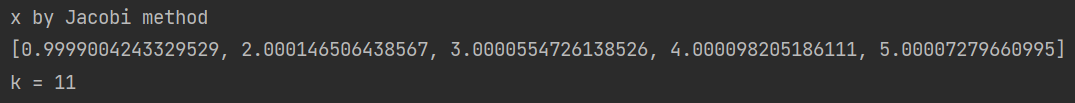
\includegraphics[width=0.8\textwidth]{img1}
\caption{Вектор x и число итераций метода Якоби}
\label{fig:img1}
\end{figure}

\begin{figure}[!htb]
	\centering
	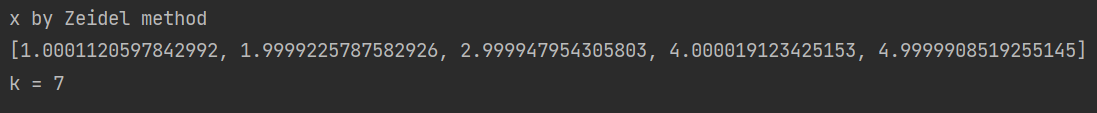
\includegraphics[width=0.8\textwidth]{img2}
\caption{Вектор x и число итераций метода Зейделя}
\label{fig:img2}
\end{figure}

\section{Выводы}\label{Sect::conclusion}

В результате выполнения лабораторной работы был реализован метод Зейделя.
\end{document}
